
\subsection{Source Datasets}

\begin{figure}[t]
  \centering
  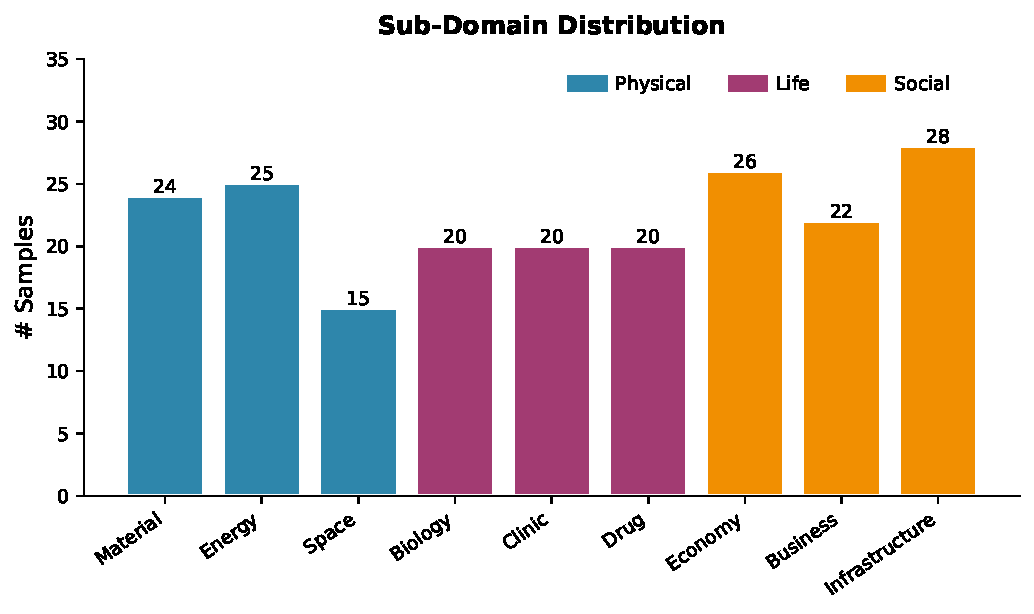
\includegraphics[width=0.8\linewidth]{figures/eywabench/fig1b_subdomain_bar.pdf}
  \caption{Composition of \textit{Eywabench} along sub-domains. distributions are all near-uniform, avoiding the domain-collapse failure modes.}
  \label{fig:eywa_overview}
\end{figure}




\textit{EywaBench} currently consists of 4 datasets: DeepPrinciple \cite{song2025evaluating}, MMLU-Pro \cite{wang2024mmlu}, fev-bench \cite{DBLP:journals/corr/abs-2509-26468}, and TabArena \cite{DBLP:journals/corr/abs-2506-16791}.

\textbf{DeepPrinciple: scientific QA dataset.} 
A scenario-grounded benchmark for authentic scientific discovery across four core disciplines (biology, chemistry, materials science, and physics). It advances beyond decontextualized QA by introducing a large-scale, two-phase evaluation that requires agents to perform iterative reasoning, hypothesis generation, and experimental design in highly diverse scientific contexts.

\textbf{MMLU-Pro: multi-task language understanding benchmark.}
A substantially enhanced reasoning benchmark comprising over 12,000 carefully curated questions across 14 diverse domains. We select scientific domains and convert the original multiple-choice format into open-ended question answering, requiring models to produce direct answers.


\textbf{fev-bench: realistic large-scale time series dataset.}
A comprehensive time series forecasting benchmark containing ~100 rigorous time series. Many of the time series incorporate complex, realistic covariates, which further highlight their high diversity.

\textbf{TabArena: large-scale tabular dataset.}
A curated collection of 51 tabular classification and regression datasets covering a wide array of real-world use cases. Supported by a massive evaluation scale of approximately 25 million trained model instances, it offers immense diversity in feature spaces and data distributions for tabular machine learning.


\begin{figure*}[t]
  \centering
  \begin{subfigure}[t]{0.49\linewidth}
    \centering
    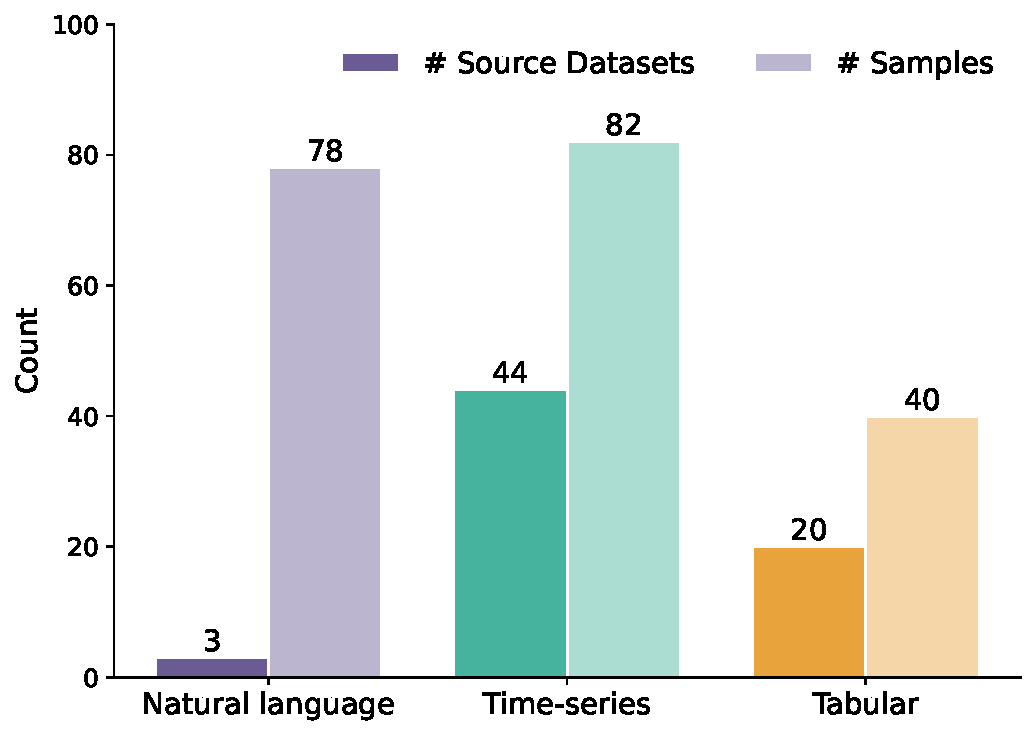
\includegraphics[width=\linewidth]{figures/eywabench/fig5a_source_modality_counts.pdf}
    \caption{Source-dataset and sample counts by modality.}
    \label{fig:source_modality_counts}
  \end{subfigure}\hfill
  \begin{subfigure}[t]{0.49\linewidth}
    \centering
    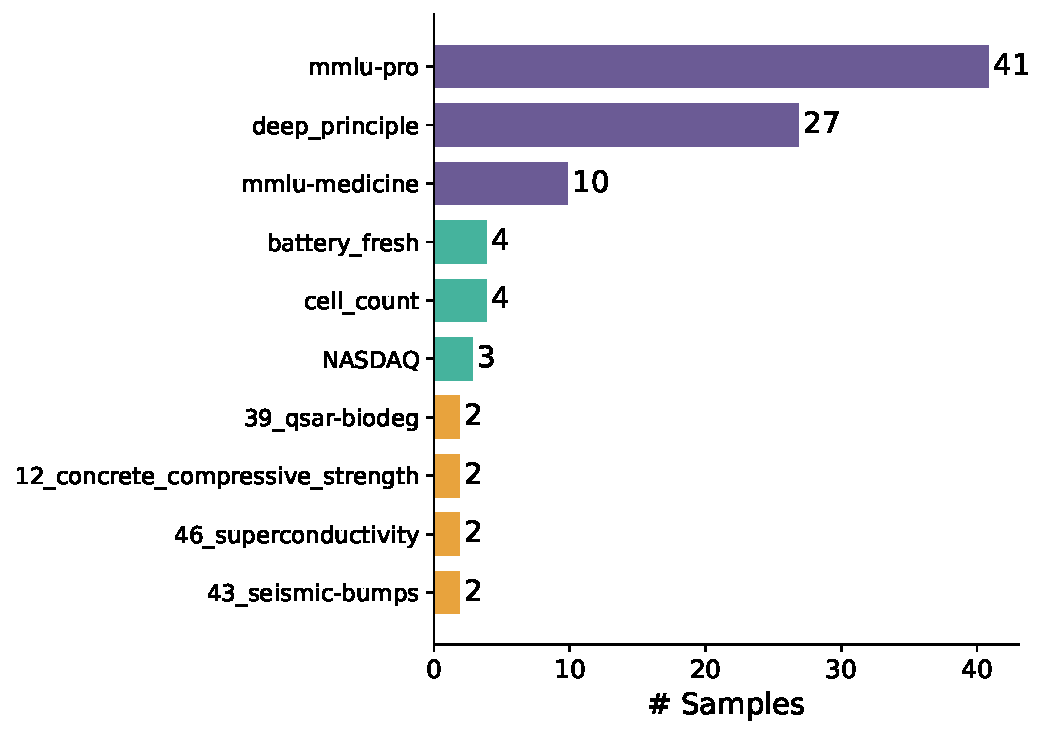
\includegraphics[width=\linewidth]{figures/eywabench/fig5b_top_source_datasets.pdf}
    \caption{Top-10 source datasets by sample count.}
    \label{fig:top_source_datasets}
  \end{subfigure}
  \caption{Source diversity of \textit{EywaBench-V1}. 
  (a) The benchmark covers distinct source datasets and task samples across natural-language, time-series, and tabular modalities, showing broad modality-level coverage. 
  (b) The top-10 source datasets follow a long-tailed distribution, with no single source dominating the benchmark. 
  This design reduces the risk that method rankings are driven by overfitting to a single source distribution.}
  \label{fig:eywa_sources}
\end{figure*}


\textbf{Scalability and Sampling.}
\textit{EywaBench} is designed to be scalable. Its source tasks are drawn from large and diverse scientific benchmarks: DeepPrinciple contains 1,125 questions spanning chemistry, materials science, biology, and physics; MMLU-Pro contains 6,978 questions across physics, chemistry, engineering, economics, health, business, biology, and computer science; FEV-Bench includes 96 time-series datasets, each with up to 30,000 covariate series; and the tabular benchmark contains 51 tables, each with up to 150,000 rows. Moreover, for time-series and tabular tasks, additional task instances can be constructed by sampling different sub-series, covariate groups, rows, columns, and prediction targets from the original datasets. This makes the potential scale of \textit{EywaBench} substantially larger than the number of original datasets alone.

\textbf{\textit{EywaBench-V1.}}
In this work, we sample 200 task instances from the four benchmark sources to form a controlled evaluation subset. This choice is motivated by two considerations. First, unlike standard language-only benchmarks, evaluating heterogeneous agentic systems requires manually configuring and validating \textit{EywaMAS}. Exhaustively evaluating all possible task instances would therefore be prohibitively expensive for human expert inspection. Second, a moderate-sized subset allows us to maintain balanced coverage across domains and data modalities while keeping the evaluation reproducible and comparable across different agentic frameworks.


\subsection{Data Schema}

\begin{table}[h]
    \centering
    \caption{Data schema of \textit{EywaBench}. The benchmark is stored as a dictionary-encoded Parquet file with 200 task instances and six fields.}
    \label{tab:eywabench_schema}
    \resizebox{0.9\linewidth}{!}{
    \begin{tabular}{lll}
        \toprule
        \textbf{Column} & \textbf{Type} & \textbf{Description} \\
        \midrule
        \texttt{domain} & categorical & Scientific sub-domain, e.g., materials, energy, biology. \\
        \texttt{task} & string & Task type associated with the sample. \\
        \texttt{description} & string & Detailed task description of the sample. \\
        \texttt{output\_size} & int64 & Maximum allowed output length for the solver. \\
        \texttt{input} & string & Prompt, context, or structured input provided to the solver. \\
        \texttt{label} & string & Ground-truth output or reference answer. \\
        \bottomrule
    \end{tabular}
    }
\end{table}


\textit{EywaBench-V1} is released as a single self-contained Parquet file. The file is dictionary-encoded with Snappy compression and generated using PyArrow~20.0.0 and pandas~2.3.3. Each row represents one self-contained scientific problem and follows the six-column schema summarized in Table~\ref{tab:eywabench_schema}. For each source dataset, we also provide parsing scripts that convert its original data format into the unified \textit{EywaBench} schema.


\subsection{Composition and Coverage Analysis}
\label{sec:eywabench_analysis}


All statistics in this section are computed directly from the \textit{EywaBench-V1} parquet split.

\textbf{Overview.}

\begin{figure}[t]
  \centering
  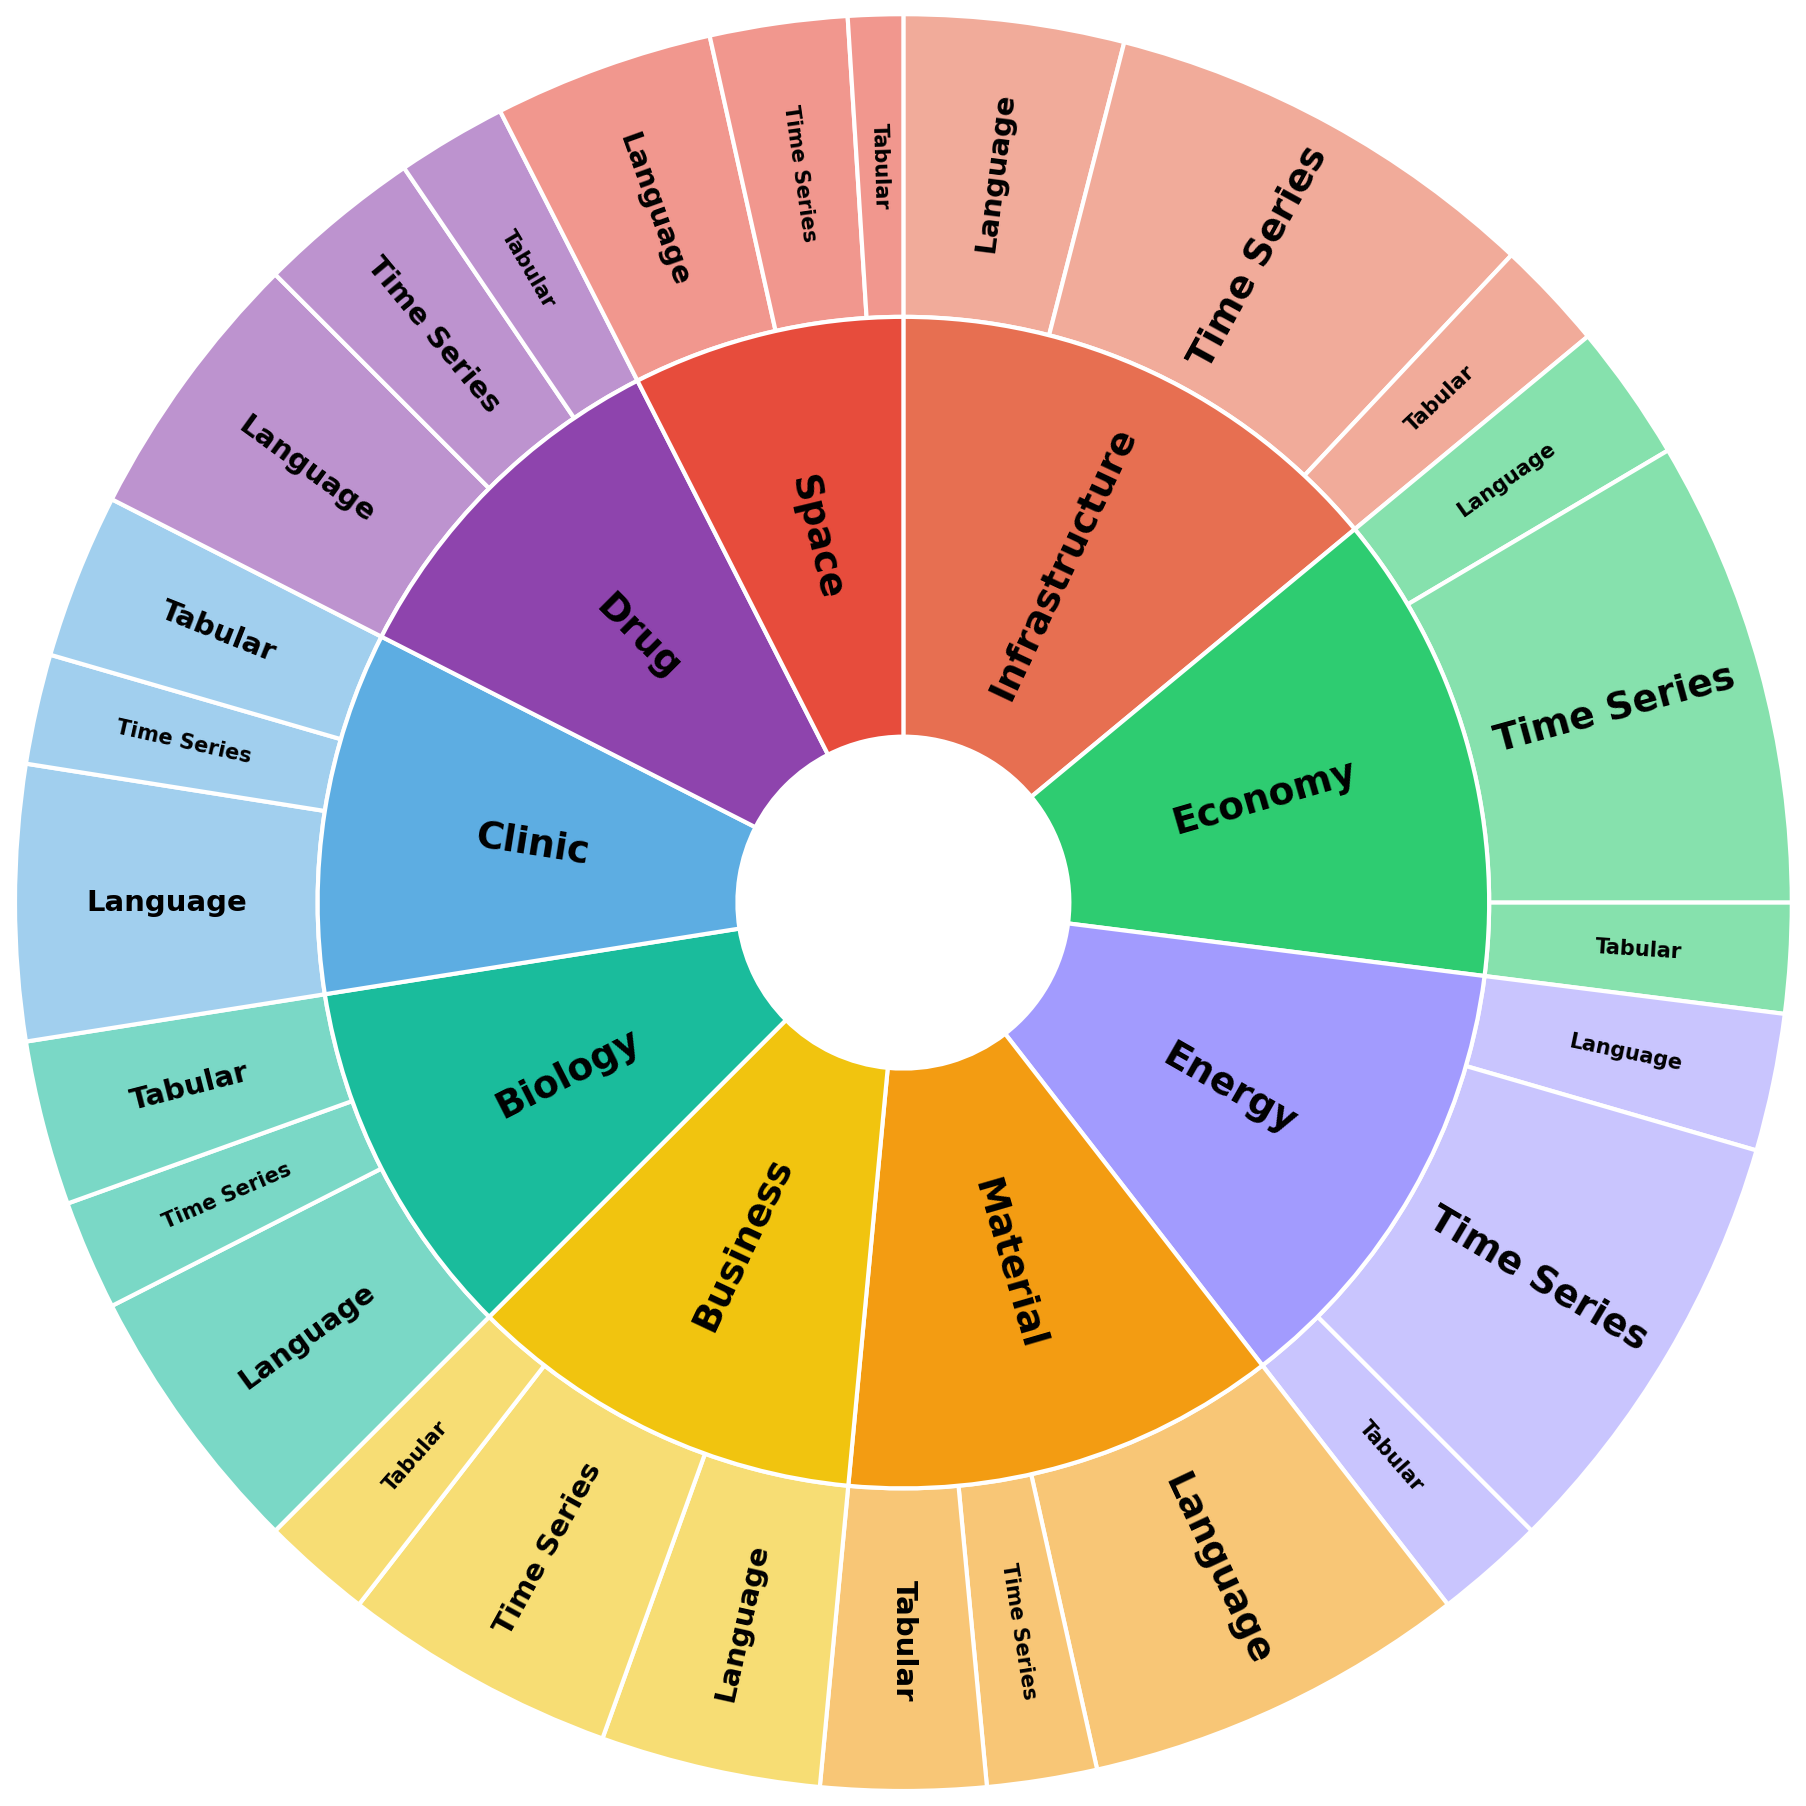
\includegraphics[width=0.6\linewidth]{figures/fig_sunburst_modality.jpg}
  \caption{Hierarchical view of \textit{Eywabench}: nine sub-domains
(inner ring) $\times$ three modalities (outer ring). All $27$
cells are populated; the largest sub-domain accounts for $14.0\%$
of the benchmark.}
  \label{fig:eywa_hierarchy}
\end{figure}

The released split contains $N{=}200$ task samples. The underlying construction pipeline is fully parametric and can be scaled along two independent axes: (i)~\emph{sample volume}, where additional instances can be generated from the same source datasets by resampling temporal windows, tabular subsets, covariate groups, or prediction targets without changing the benchmark schema; and (ii)~\emph{domain and modality coverage}, where new scientific domains and data modalities can be incorporated through additional parsers. Therefore, the released split should be viewed as a \emph{representative slice} of a much larger and extensible benchmark space.


\paragraph{Balanced taxonomy along three orthogonal axes.}
\textit{Eywabench} is organised as a three-tier taxonomy (parent domain~$\to$~sub-domain~$\to$~source dataset), and is simultaneously stratified along the modality axis. The benchmark is near-uniform along all three principal axes: the three parent domains are covered at $32.0\%/30.0\%/38.0\%$, the nine sub-domains each contain $15$--$28$ instances, and the modalities are represented at $41.0\%/39.0\%/20.0\%$. We provide a visualization in Figure~\ref{fig:eywa_overview}. Quantitatively, the normalised Shannon entropy (where $H_{n}{=}1$ denotes a perfectly uniform distribution) is $H_{n}{=}0.995$ at the parent level, $H_{n}{=}0.993$ at the sub-domain level, and $H_{n}{=}0.960$ at the modality level, indicating that no single domain or modality dominates the benchmark.
every one of the nine sub-domains carries a non-trivial mix of all three modalities, yielding $100\%$ cross-modal coverage of the taxonomy. This ensures that conclusions about modality-specific agent behaviour drawn from \textit{Eywabench} generalise across scientific fields rather than conflating modality effects with domain effects. We provide a modality visualization in Figure \ref{fig:eywa_hierarchy}.

% ----------------- Detailed sub-domain table ------------------------
\begin{table}[h]
\centering
\caption{Detailed composition of \textit{EywaBench-V1} by parent domain, sub-domain, modality, and source dataset. 
For each sub-domain, we report the total number of samples, the number of natural-language, time-series, and tabular samples, and the number of distinct source datasets. 
The total number of unique source datasets is $67$, which is smaller than the sum of per-sub-domain source counts because each source dataset may contribute multiple samples.}
\label{tab:eywa_subdomain}
\resizebox{0.85\linewidth}{!}{%
\begin{tabular}{llccccc}
\toprule
\textbf{Parent} & \textbf{Sub-domain} & \textbf{\# samples} & \textbf{Natural Language} & \textbf{Time Series} & \textbf{Tabular} & \textbf{\# Source Datasets} \\
\midrule
\multirow{3}{*}{Physical}
 & Material       & $24$ & $14$ & $4$  & $6$ & $5$  \\
 & Energy         & $25$ & $5$  & $16$ & $4$ & $11$ \\
 & Space          & $15$ & $8$  & $5$  & $2$ & $7$  \\
\midrule
\multirow{3}{*}{Life}
 & Biology        & $20$ & $10$ & $4$  & $6$ & $5$  \\
 & Clinic         & $20$ & $10$ & $4$  & $6$ & $6$  \\
 & Drug           & $20$ & $10$ & $6$  & $4$ & $9$  \\
\midrule
\multirow{3}{*}{Social}
 & Economy        & $26$ & $5$  & $17$ & $4$ & $11$ \\
 & Business       & $22$ & $8$  & $10$ & $4$ & $8$  \\
 & Infrastructure & $28$ & $8$  & $16$ & $4$ & $11$ \\
\midrule
\multicolumn{2}{l}{\textbf{Total}} & $\mathbf{200}$ & $\mathbf{78}$ & $\mathbf{82}$ & $\mathbf{40}$ & $\mathbf{67}$ \\
\bottomrule
\end{tabular}}
\end{table}


\paragraph{Diversity of source datasets.}
At the leaf level of the taxonomy, \textit{EywaBench-V1} draws samples from $67$ distinct source datasets. These sources cover a broad range of scientific data, including ETT, ERCOT, NASDAQ, Jena Weather, LOOP-SEATTLE, Concrete Compressive Strength, and Superconductivity, among others. Overall, the benchmark includes $21$ physical-science sources, $19$ life-science sources, and $28$ social-science sources. The source distribution has a normalized Shannon entropy of $H_n{=}0.846$, indicating high diversity with a long-tailed structure, as visualized in Figure~\ref{fig:eywa_sources}. Importantly, even the largest individual source, MMLU-Pro, contributes only $41$ samples, accounting for $20.5\%$ of the benchmark. This reduces the risk that method rankings are dominated by any single source distribution.


\subsection{Metrics}
\label{sec:metrics}

Each task instance $i$ produces a per-instance \emph{utility} $u_i \in [0,1]$ ($u_i{=}1$ for a perfect prediction). Because \textit{EywaBench} mixes three output modalities, $u_i$ is defined modality-specifically while always being bounded in $[0,1]$ so that scores are directly comparable across modalities. Slice-level numbers reported in the paper are the unweighted mean $\bar{u}(\mathcal{D}) = \tfrac{1}{|\mathcal{D}|}\sum_{i\in\mathcal{D}} u_i$ (with sample standard deviation as dispersion); the same aggregation is applied to runtime and the four token-cost components.

\textbf{Natural language.}
For DeepPrinciple and the open-ended MMLU-Pro variant, the raw output is first reduced to a final answer $\hat{y}_i$ and normalised by an operator $\pi$ that trims whitespace/quotes, collapses inner whitespace, and maps a few Unicode variants to ASCII. We then apply a three-stage soft-score cascade:
\emph{(i) Exact match.} If $\pi(\hat{y}_i)=\pi(y_i)$, set $u_i{=}1$.
\emph{(ii) Numeric relative error.} If both sides parse as a single float $\hat{p},g$, set
\begin{equation}
u_i = \exp(-e_{\mathrm{rel}}), \qquad e_{\mathrm{rel}} = \frac{|\hat{p}-g|}{\max(|g|,\,10^{-12})}.
\label{eq:nl_numeric}
\end{equation}
\emph{(iii) Lexical fallback.} Otherwise tokenise both strings with a regex that preserves \LaTeX{} commands, words, numbers, and individual symbols; let $o$ be the multiset overlap and define token precision/recall/F1 as $P_\mathrm{tok}{=}o/|T_\mathrm{pred}|$, $R_\mathrm{tok}{=}o/|T_\mathrm{gold}|$, $F_1^{\mathrm{tok}}{=}2P_\mathrm{tok}R_\mathrm{tok}/(P_\mathrm{tok}{+}R_\mathrm{tok})$ (with $F_1^{\mathrm{tok}}{=}1$ if both empty and $0$ if exactly one is empty). Let $S_\mathrm{char}$ be the \texttt{difflib.SequenceMatcher} ratio on the normalised strings. Then
\begin{equation}
u_i = \min\!\bigl(\tau,\; \alpha\,F_1^{\mathrm{tok}} + \beta\,S_\mathrm{char}\bigr), \qquad \alpha{=}0.6,\ \beta{=}0.4,\ \tau{=}0.8.
\label{eq:nl_textual}
\end{equation}
The cap $\tau$ keeps lexical near-misses strictly below the scores reserved for stages (i)--(ii).

\textbf{Time series.}
The gold and predicted continuations $\mathbf{y},\hat{\mathbf{y}}\in\mathbb{R}^{H}$ are parsed from \texttt{(timestamp,value)} CSVs. With a denominator floor $\varepsilon{=}10^{-2}$ and $\mathcal{I}{=}\{t:|y_t|{>}\varepsilon\}$,
\begin{equation}
\mathrm{sMAPE} = \frac{1}{H}\sum_{t=1}^{H} \frac{2|y_t-\hat{y}_t|}{\max(|y_t|+|\hat{y}_t|,\varepsilon)} \in [0,2], \qquad
\mathrm{MAAPE} = \frac{1}{|\mathcal{I}|}\sum_{t\in\mathcal{I}} \arctan\!\frac{|y_t-\hat{y}_t|}{\max(|y_t|,\varepsilon)} \in [0,\pi/2],
\label{eq:smape_maape}
\end{equation}
($\mathrm{MAAPE}{=}0$ when $\mathcal{I}{=}\emptyset$). The two errors are normalised to $[0,1]$ and combined into
\begin{equation}
u_i = 1 - \frac{1}{2}\!\left(\frac{\mathrm{sMAPE}}{2} + \frac{\mathrm{MAAPE}}{\pi/2}\right) \in [0,1].
\label{eq:ts_utility}
\end{equation}
Combining the two mitigates the pathologies of either metric used alone: $\mathrm{sMAPE}$ saturates symmetrically but is brittle near zero, whereas $\mathrm{MAAPE}$ is well-behaved near zero but less scale-sensitive.

\textbf{Tabular.}
The label and prediction strings are parsed into 1-D arrays via \texttt{DataFrame.values.flatten()} (or \texttt{eval} when the string starts with \texttt{[}). For classification tasks the utility is top-1 accuracy,
\begin{equation}
u_i = \frac{1}{N}\sum_{n=1}^{N} \mathbf{1}\!\bigl[\hat{y}_n = y_n\bigr],
\label{eq:tab_cls}
\end{equation}
implemented via \texttt{sklearn.metrics.accuracy\_score}. For regression tasks the predicted and gold target columns are scored with the same sMAPE+MAAPE combination as time series (Eqs.~\eqref{eq:smape_maape}--\eqref{eq:ts_utility}), treating the $N$ row-wise predictions as an $H$-step forecast. Sharing this rule across modalities keeps numeric-target errors on a common scale, so the cross-modal averages reported in the main paper are directly comparable.